All 16 declared cases completed with the fixed call quota. A counted 11, 12, 9, and 9 on the four clips in each repeat; B counted 12, 11, 11, and 12. Each repeat therefore had MAE 1.50 for A and 0.25 for B, with exact agreement in one and three of four videos, respectively. B's August~15 underestimate is retained: the policy did not improve every clip.

Each policy used 1,030 non-warm-up calls per repeat, plus four separate warm-ups. Across both repeats B allocated 66 calls to local crops and 1994 to global images; A used 2060 global calls. All 4,120 non-warm-up raw arrays were checked against their call records. The independent comparison of 24 pairs of runs found 6,015 shared global input/output hash pairs, all identical; the pair count is not additional independent observations.

The event-publication maximum over all runs was 986.286~ms. The observation-completion maximum was 1141.255~ms, and the largest per-run observation p95 was 927.872~ms. Capture lateness reached 250.315~ms and final stream drain reached 0.615752~s. All original replay reference checks passed, including the 1,500-ms observation maximum; not every observation was younger than 1~s. Acquisition remained paced, all admitted calls used arrived frames, and no planned global was lost in this block.

\begin{figure*}[!t]
\centering
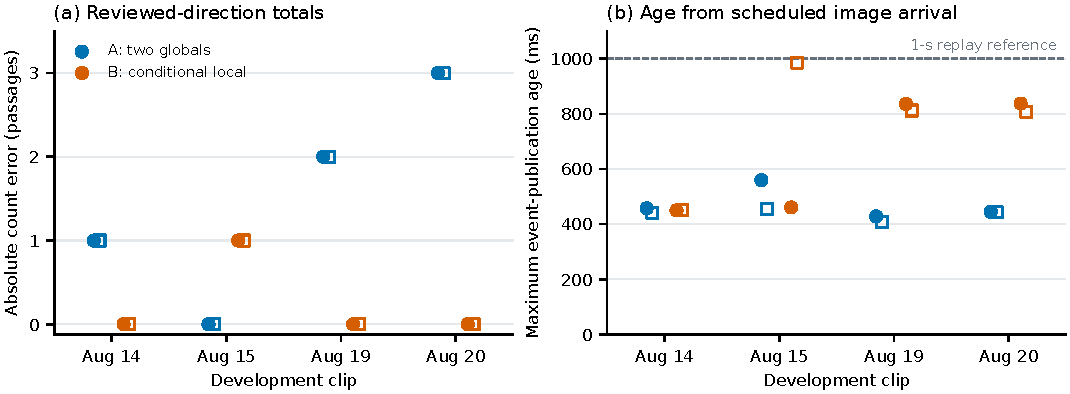
\includegraphics[width=0.98\textwidth]{figures/paired_results.pdf}
\caption{Count error and maximum event-publication age for all sixteen development replays. Filled circles and open squares indicate repeats 1 and 2; they are repeated executions of four videos, not additional animal samples. The 1-s line is a replay publication reference, not a measured physical crossing deadline.}
\label{fig:results}
\end{figure*}
